\documentclass[11pt]{article}
\usepackage[top=1.00in, bottom=1.0in, left=1in, right=1in]{geometry}
\renewcommand{\baselinestretch}{1.1}
\usepackage{graphicx}
\usepackage{natbib}
\usepackage{amsmath}

\begin{document}
\bibliographystyle{/Users/Lizzie/Documents/EndnoteRelated/Bibtex/styles/besjournals}
\renewcommand{\refname}{\CHead{}}

\hspace{-5ex} \includegraphics[width=0.5\textwidth]{/Users/Lizzie/Documents/Professional/images/letterhead/ubc/Faculty of forestry.png}
\pagenumbering{gobble}
\vspace{1.5ex}\\

\setlength{\parindent}{0pt}
\setlength{\parskip}{7pt}
\today

% To JD (23 July 2024):
% Would you take a quick look at my pre-submission inquiry for TREE? I am trying to meet the requirements here (not sure if point by point means bullet points, but I added them): https://www.cell.com/trends/ecology-evolution/presubmission
% I also tried to echo their aims and scopes: https://www.cell.com/trends/ecology-evolution/aims 

Dear Dr. Stephens:

We would like to propose an \emph{Opinion} for \emph{Trends in Ecology \& Evolution} entitled `A four-step Bayesian workflow for improving ecological science.' % ... and show how it can enhance data collection, forecasting, and statistical training.  % The workflow is designed to be broadly generalizable and practical. To make sure the steps are clear and accessible we would present full example of the workflow and accompanying code (in R Markdown) to estimate trends over time in plant and animal phenology. 
Given the increasing aims of forecasting and prediction today, ecologists are using more complex models to leverage larger datasets \citep{anderson2021trends,muff2022rewriting}, but many researchers---ourselves included---were not trained in best statistical practice for these approaches. This  can lead to poor models and incorrect predictions and decisions. While the field of statistics has worked to develop robust workflows for analysing complex data, these advances have largely failed to percolate into ecological and evolutionary research.% However, while many ecologists may not be formally trained in the fitting of large, complex models, they often have the computational toolkit to approach such models, but lack an organizational framework to develop, test and improve bespoke models. 
\begin{itemize}
\item To bridge this gap, we outline a generalizable workflow for ecological and evolutionary research (see Fig. \ref{fig:workflow} below), which is built on fundamental scientific principles and new insights from statistics and data science \citep[][]{grinsztajn2021,vandeschoot2021}. This approach  moves away from a focus on null hypothesis testing, towards estimating effect sizes, with models calibrated and better understood through simulating data at multiple steps---using a number of skills more often associated with theoretical than empirical ecology. We conclude by highlighting how adopting this workflow may improve statistical and mathematical training in ecology, including how we implement machine learning models and other new approaches. 
\item There have been many in-depth articles on various aspects of model fitting and validation in recent years \citep[e.g.][]{conn2018,gabryvis,tredennick2021practical,direnzo2023practical}, but there have been no attempts---to our knowledge---to generate a statistical workflow aimed directly at evolutionary biologists and ecologists. While we build on recent advances in scientific and statistical workflows in other disciplines \citep{gelman2020bayesian,grinsztajn2021,schad2021}, we provide a unique perspective by explaining the workflow and why it is both tractable and critical now for ecological and evolutionary science. 
\item We believe this article would be ideal for \emph{TREE} given our aims for it to be concise and extremely approachable. The workflow is designed to be generalizable across disciplines of ecology and evolution. To make sure the steps are clear and accessible we would present a full example of the workflow and accompanying code (in R Markdown) to estimate trends over time in plant and animal phenology. 
\end{itemize}

% Fitting larger and sometimes more complex models presents challenges that can be overcome by approaching analyses through specific workflows \citep{betanworkflow,grinsztajn2021,vandeschoot2021}, which themselves are built on a process of how to do not just statistics, but how to do science \citep{box1976science}. Such approaches move away from a focus on null hypothesis testing, towards estimating effect sizes, using models calibrated and better understood through simulating data at multiple steps---using a number of skills often reserved in ecology more for `theorists' than empirical ecologists. But this theoretical-vs-empirical divide ignores that the average modern ecologist is computational, and thus already has many of the basic skills to build bespoke models. 
% We then outline one such iterative workflow, which contains four steps (see Fig. \ref{fig:workflow} below), highlighting how it has changed our science and how it may alter statistical and mathematical training in ecology. These steps include discussion (and definitions) of model calibration, non-identifiability, prior predictive checks, power analyses through simulation and iterative model building. 

The manuscript is authored by an international and interdisciplinary group of ecologists, evolutionary biologists and statisticians. The workflow follows the basics of how authors EM Wolkovich, TJ Davies (UBC) and WD Pearse (Imperial College) approach model building, and leverages the insights and skills of computational statistician M Betancourt (Symplectomorphic LLC) who has developed fundamental statistical workflows for diverse scientific disciplines. We realize our author list is one person beyond the desired size, but we found multiple perspectives on how to implement this workflow have been especially useful. % We have designed it to be broadly generalizable and practical, including relevant examples of forecasting shifts in animals and plants over time.

We hope that you will find our proposed submission, which provides a road-map for the many ecologists now building more complex models, suitable for publication in \emph{Trends in Ecology \& Evolution}. By integrating simulation more fully in model building and testing this workflow can help fit models that are more robust and well-suited to provide new ecological insights---allowing us to refine where to put resources for better estimates, better models, and better forecasts. % This manuscript is not under consideration elsewhere, and all authors approved of this version for submission. 

Sincerely,\\

\includegraphics[scale=1]{/Users/Lizzie/Documents/Professional/Vitas/Signatures/SignatureLizzieSm.png} \\

Elizabeth M Wolkovich\\
Associate Professor of Forest \& Conservation Sciences\\ 
University of British Columbia\\

{\bf Relevant recent articles:}

As we mention above, our article leverages advances in statistical workflows, which were developed especially by more Bayesian-focused statisticians,  but designed to be applicable widely \citep{betanworkflow,gelman2020bayesian}. These new approaches have been adapted to epidemiology and cognitive science  \citep{grinsztajn2021,schad2021}; our article would be the first to introduce them specifically to evolutionary and ecological research. We believe an approachable, concise treatment of this workflow may be especially powerful in ecology where many researchers now have the computational toolkit to fit larger more complicated models, but lack an organizational framework on how best to develop, test and improve their models. By adopting a standardised workflow, such as the one we propose, we hope more ecologists will be confident to fit their data to bespoke mathematical models of biological systems, which in turn would yield better inference, predictions and forecasts. 

\newpage
{\bf Example figure}

\begin{figure}[ht]
\centering
\noindent 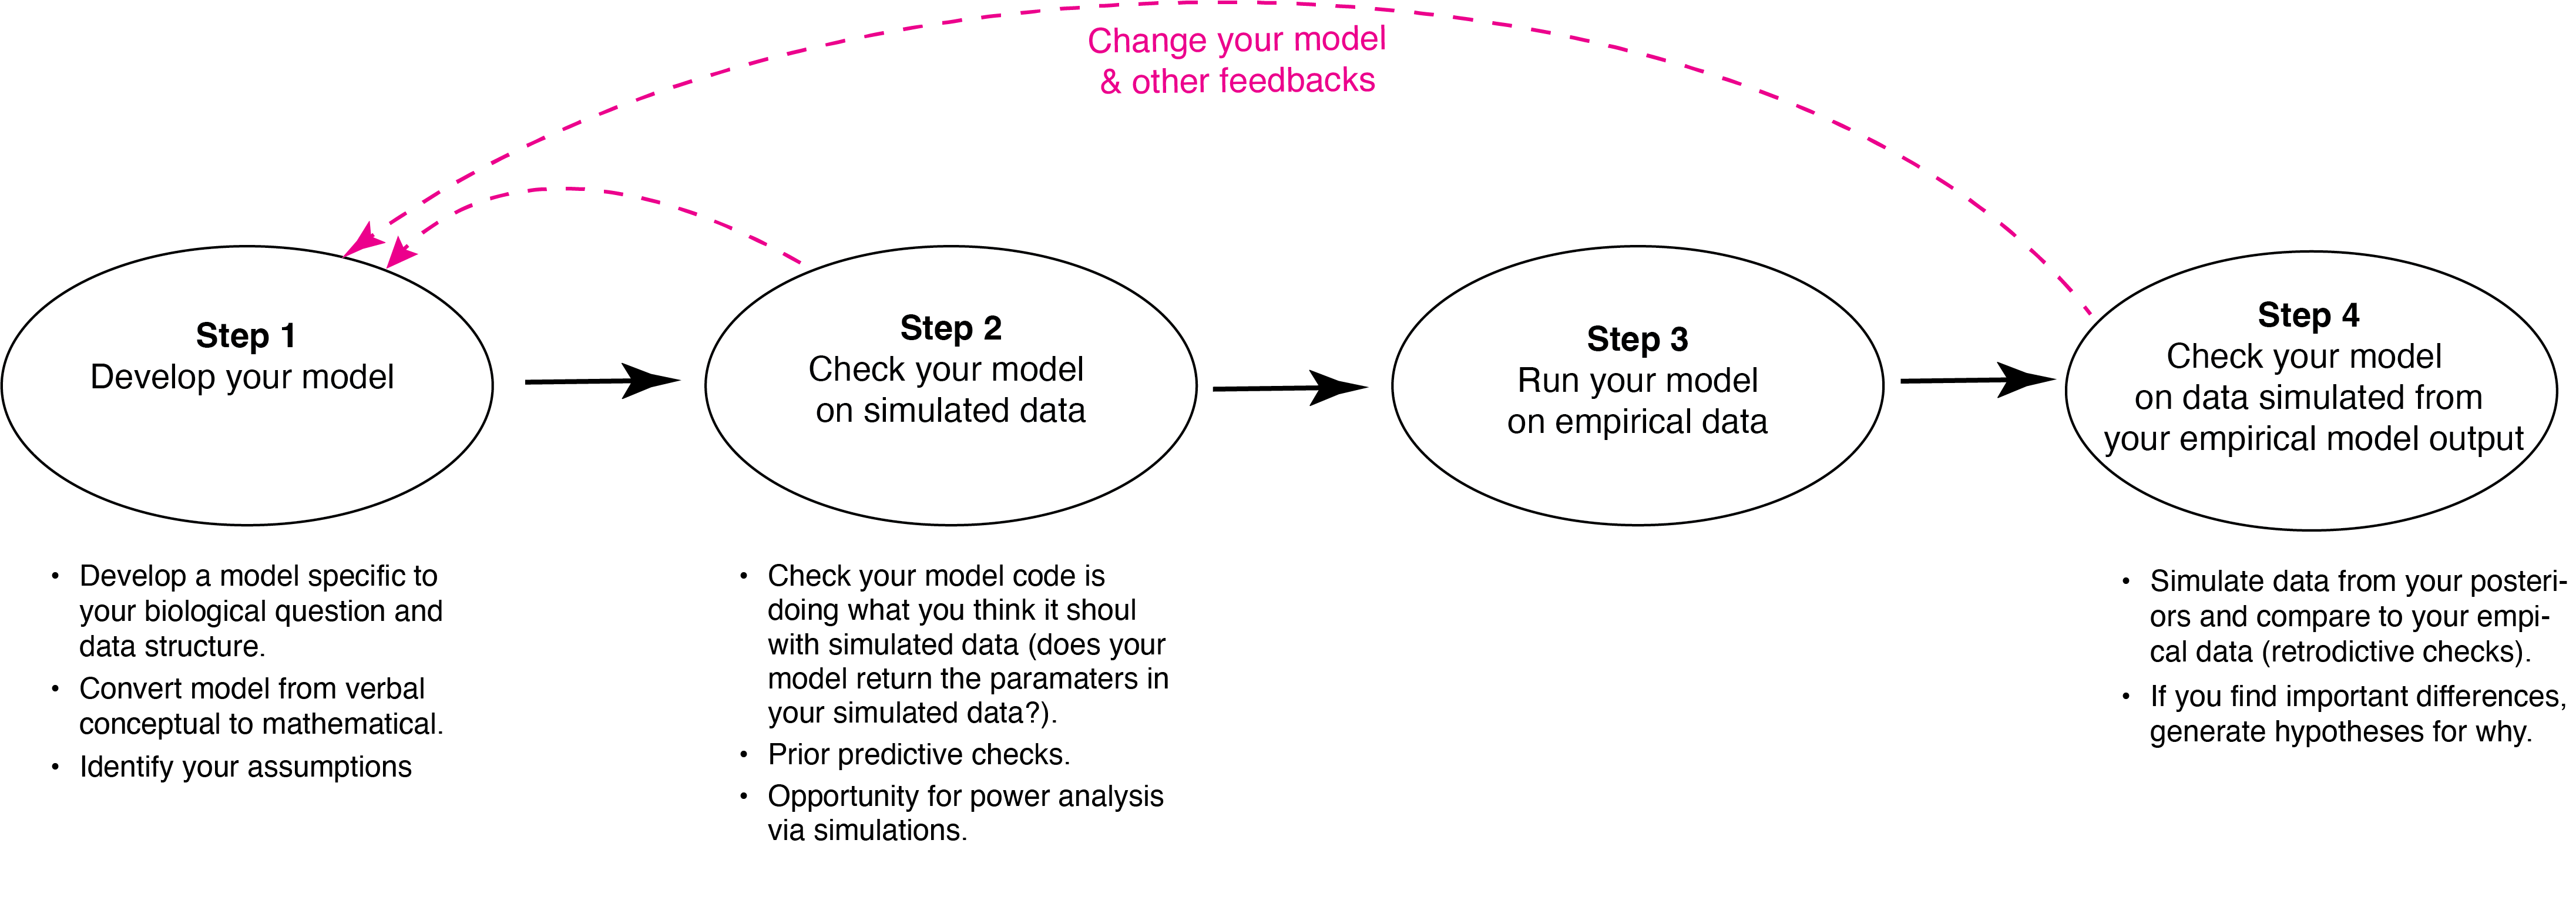
\includegraphics[width=1\textwidth]{..//figures/workflow.png}
\caption{The four-step iterative workflow we outline can help design models for specific ecological questions, data and aims---which makes this a statistical workflow that can naturally become a scientific workflow. It makes the step that many of us focus on---running your model on your empirical data (Step 3)---far more straightforward and insightful by using simulations both before (Step 2) and after (Step 4) it to better understand the model and data together.}
\label{fig:workflow}
\end{figure}

\newpage
{\bf References}
\vspace{-4ex}
\bibliography{..//refs/bayesrefsmini.bib}

\end{document}





%%%
%%%

\begin{figure}[ht]
\centering
\noindent 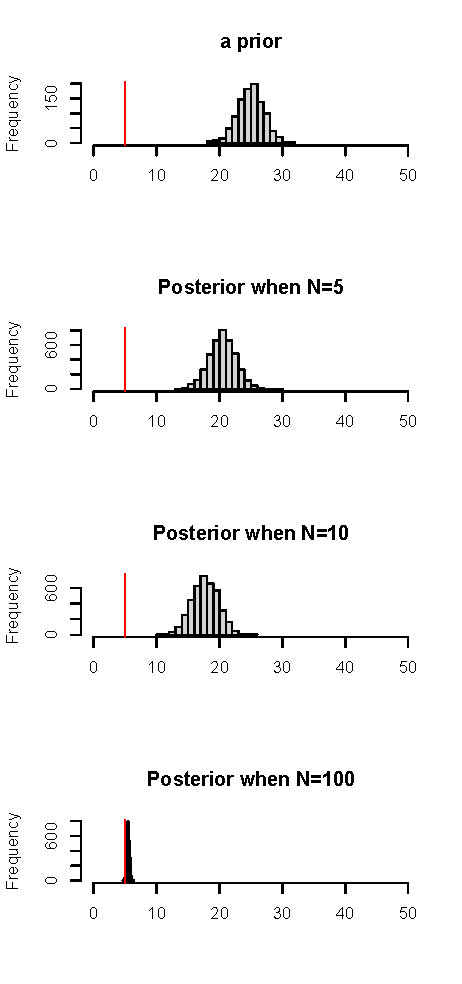
\includegraphics[width=0.5\textwidth]{..//examples/misspecifiedmodel/priorpostforflows.pdf}
\caption{A simple example of how to use simulated data to understand calibration issues in a mis-specified model. Here we know the true model underlying the data is $y=\alpha + \text{normal}(0, \sigma)$ where $\alpha$ is 5 (shown as blue vertical line) and $\sigma$ is 2. The model, however, is mis-specified by a prior for $\alpha$ of $\text{normal}(25, 2)$ (dashed blue line), resulting in a posterior (salmon-colored histogram) not centered on the true value. In our experience it is quite rare to have a prior informed by ecological knowledge be so far off, but this is an example. How mis-calibrated the model will be depends on the data: we show examples with a sample size ($N$) of 5, 10 and 40 data points. In practice these studies would allow us to determine how much data we would need to be robust to suspect prior models. (Note the change in $y$ axis range for bottom plot.) }
\label{fig:misspecifyprior}
\end{figure}


